\begin{frame}{ALgorithme de prétraitement}
\begin{figure}
    \centering
    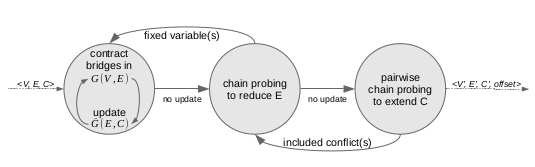
\includegraphics[width=0.9\textwidth]{img/peprocessing.png}
\end{figure}
    

\begin{block}{étapes}
\begin{enumerate}
    \item  Une contraction dans la première étape des arêtes pont(bridges).
    \item une suppression d'arête $e$ tel que $\delta_{ \hat{G}}(e) > 0 $, si la suppression de ses arêtes en conflits déconnecte le graphe, puis mise à jour de C.
    \item Choisir $e_{1},e_{2}$ tel que $\{e_{1},e_{2}\} \not\in C$ , si la suppression de leurs conflits déconnecte le graphe alors ajouter $\{e_{1},e_{2}\} \in C$ .
\end{enumerate}
   

\end{block}

\end{frame}
\begin{frame}{Algorithme de prétraitement}
\begin{block}{phase 01}

\end{block}

    
\end{frame}

\begin{frame}{Algorithme de prétraitement}
\begin{block}{Phase 02}
 \forall $ e_{i},e_{j}   \not\in C $, $\delta_{ \hat{G}}(e) > 0 $, ajouter \{$e_{i},e_{j}\} \in C$\quad SSI \quad G'=(V, E') est non connexe avec E'=E/$\{e_{i},e_{j}\}$
\end{block}

\textbf{Démonstration par l'absurde}
\newline
Supposant que $x_{e_{i}}=1$ \quad \textbf{$\Rightarrow $} \quad   $e_{j}=0$ car $\{e_{i},e_{j}\} \in S $; 
\newline Or $G/\{e_{j}\}$ non connexe.
\newline \textbf{contradiction} avec $X^*$ est un arbre.
\end{frame}
\begin{frame}{Algorithme de prétraitement}
\begin{block}{phase 03}
\forall $ e_{i},e_{j} \in E $\; Tq $\{e_{i},e_{j}\} \not\in C. $\newline
Soit $\chi(e_{i})$ et  $\chi(e_{j})$ l'ensemble des arêtes en conflit de $e_{i}$ et $e_{j}$ respectivement.
si G/$\chi(e_{i}) \cup \chi(e_{j})$ n'est pas connexe alors ajouter $\{e_{i},e_{i}\} \in S $
\end{block}
\textbf{Démonstration  par l'absurde}

    
\end{frame}